%\documentclass[14pt,aspectratio=169]{beamer}
\documentclass[14pt]{beamer}
\usepackage{ctex}
\usepackage{bm}
\usepackage{color, colortbl}
\usepackage{graphicx}
\graphicspath{ {./images/} }
\setbeamertemplate{caption}{\raggedright\insertcaption\par}

\definecolor{HRed}{rgb}{1,.2,.2}
%\usepackage{xeCJK} % important! Without this Chinese fonts won't show
%\usepackage{xeCJKfntef}
\setsansfont{Noto Sans CJK SC Light}
\setCJKsansfont[ItalicFont=Kaiti SC]{Noto Sans CJK SC Light}
\setCJKmainfont{Noto Serif CJK SC Light}

\usefonttheme[onlymath]{serif} % formulars in serif font
\usefonttheme{professionalfonts} % 防止公式间距异常,参见https://www.zhihu.com/question/55492768
\parskip=10pt

%\newcommand{\mat}[1]{\bm{#1}}
\newcommand{\mat}[1]{\bm{#1}}
\renewcommand{\vec}[1]{\bm{#1}}
\DeclareMathOperator*{\argmin}{arg\,min}

\newcommand{\MA}{\mat{A}}
\newcommand{\MI}{\mat{I}}
\newcommand{\Va}{\Vec{a}}
\newcommand{\Vy}{\vec{y}}
\newcommand{\Vx}{\vec{x}}
\newcommand{\Ve}{\vec{e}}
\newcommand{\Vw}{\vec{w}}
\newcommand{\Vt}{\vec{\theta}}
\newcommand{\SR}{\mathcal{R}}
\newcommand{\DN}{\mathcal{N}}

\let\emph\relax % there's no \RedeclareTextFontCommand
\DeclareTextFontCommand{\emph}{\color{red}\em}
\setbeamertemplate{headline}{}
\setbeamertemplate{navigation symbols}{}

%%%%%%%%%%%%%%% Section标题页 %%%%%%%%%%%%%%%%%%%%%%%
\AtBeginSection[]{
  \begin{frame}
  \vfill
  \centering
  \begin{beamercolorbox}[sep=8pt,center,shadow=true]{title}
    \usebeamerfont{title}\insertsectionhead\par%
  \end{beamercolorbox}
  \vfill
  \end{frame}
}
%%%%%%%%%%%%%%% 正文开始 %%%%%%%%%%%%%%%%%%%%%%%

\title{第10讲:Kalman滤波}
\subtitle{动态系统的线性回归}
\author{熊耀华}
\institute{交通工程系}

\begin{document}

\begin{frame}
    \titlepage
\end{frame}

\begin{frame}
  %\frametitle{Rudolf K\'alm\'an}
  \begin{figure}
    \centering
    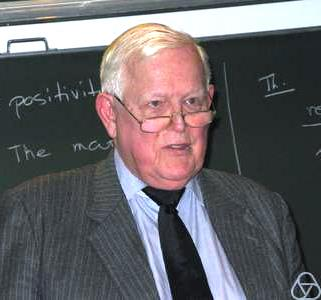
\includegraphics[width=5cm]{rudolf_kalman.jpg}
    \caption{Rudolf Emil K\'alm\'an(1930-2016)}
  \end{figure}

  \small 美籍匈牙利裔电子工程师,Kalman滤波模型的发明人。该模型传统上广泛应用于
  信号处理、控制系统、导航等领域,在新兴的所谓“大数据”领域中也有重要的地位。
\end{frame}

\begin{frame}
  \frametitle{定位问题}
  火箭发射后沿直线飞行,如何确定火箭的位置?

  {\small 火箭整体看作一个系统,系统状态为离地面距离$x$,有两种获取方式:}
  \begin{description}
    \item[地面雷达追踪] 根据火箭反射电波的飞行时间$\tau$推测距离$x$,有
    $x=c\cdot \tau/2$  
    \item[惯性导航] 火箭上的设备测量实时飞行速度$v(t)$,火箭位置为
    $x=\int v(t)dt\approx\sum v_i\Delta t=\sum \Delta x_i$
  \end{description}
\end{frame}

\begin{frame}
  \frametitle{定位误差}
  两种定位方式都有误差,但误差性质不同。对于雷达追踪
  \begin{itemize}
    \item 误差来自与计时误差
    \item 时间误差$\epsilon$带来位置误差$c\cdot\epsilon$
    \item 由于电磁波速度$c$很大,少量的计时误差也会带来显著的位置误差
    \item 两次定位相互独立,误差\emph{不累积}
  \end{itemize}
\end{frame}

\begin{frame}
  \frametitle{定位误差}
  对于惯性导航
  \begin{itemize}
    \item 误差来自速度测量,结果相对精确,对每个$\Delta x_i$只有很小的误差$e_i$
    \item 但是由于$x=\sum \Delta x_i$,总误差$\epsilon=\sum e_i$,即误差会\emph{累积}
  \end{itemize}
\end{frame}

\begin{frame}
  \frametitle{两种定位方式互补}
  两种定位方式的特点可以总结为:
  \begin{itemize}
    \item 雷达定位误差大,不累积
    \item 惯性导航误差小,累积
  \end{itemize}
  两总方式存在明显的互补性,能否\emph{融合}两种方式得到更精确的定位?
\end{frame}

\begin{frame}
  \frametitle{数据融合}
  假设第$i-1$时段的\emph{实际位置}为$\hat{x}_{i-1}$,下一个时段的位置有两个信息来源
  \begin{equation*}
    \begin{array}{ll}
      \text{预测值} & \bar{x}_i=\hat{x}_{i-1}+\Delta x_i\\
      \text{观测值} & x_i
    \end{array}
  \end{equation*}

  为了得到更准确的位置,对两个值求平均有
  \begin{equation*}
    \begin{array}{ll}
        \text{修正值}&\hat{x}_i=\frac{\bar{x}_i+x_i}{2}\\
    \end{array}
  \end{equation*}
  这个公式是否合理?
\end{frame}

\begin{frame}
  \frametitle{加权融合}
    \begin{itemize}
      \item $\hat{x}_i=\frac{\bar{x}_i+x_i}{2}=0.5\bar{x}_i+0.5x_i$假设预测值和
    修正值权重\emph{相等且不变}。
      \item 假设两者权重不等且变化可能更符合实际
      \item 此时$\hat{x}_i=a_i \bar{x}_i+b_i x_i,a_i+b_i=1$
    \end{itemize}
  
    如何确定权重$a$和$b$?
\end{frame}

\begin{frame}
  \frametitle{确定权重}
  确定权重需要简单的概率论推理。
  \begin{itemize}
    \item 假设预测值,观测值,修正值,位移都不是数字而是\emph{随机变量}
    \item 各随机变量都是正态分布,分别记为
    \begin{equation*}
      \begin{array}{rll}
        \text{预测值} && \bar{X}_i\sim \DN(\bar{x}_i, \bar{\sigma}_i^2)\\
        \text{观测值} && X_i\sim \DN(x_i, \sigma_i^2)\\
        \text{修正值} && \hat{X}_i\sim \DN(\hat{x}_i, \hat{\sigma}_i^2)\\
        \text{位移} && \Delta X_i\sim \DN(\Delta x_i, p_i^2)\\
      \end{array}
    \end{equation*}
  \end{itemize}
\end{frame}

\begin{frame}
  \frametitle{确定权重}
  此时预测步骤为
  $$\bar{X}_i=\hat{X}_{i-1}+\Delta X_i$$
  修正步骤根据贝叶斯公式,变为预测值和修正值的分布函数相乘
  $$\hat{X}_i\propto\DN(\bar{x}_i, \bar{\sigma}_i^2)\cdot
  \DN(x_i, \sigma_i^2)$$

  两个正态分布随机变量相加,两个正态分布函数相乘。正态分布的优良性质能极大的简化计算。
\end{frame}

\begin{frame}
  \frametitle{正态分布的性质}
  有两个正态分布随机变量
  $$X_a\sim\DN(\mu_a, \sigma_a^2)\qquad X_b\sim\DN(\mu_b, \sigma_b^2)$$
  如下等式成立
  \begin{align*}
    X_a+X_b&\sim \DN(\mu_a+\mu_b,\sigma_a^2+\sigma_b^2)\\
    \DN(\mu_a, \sigma_a^2)\cdot\DN(\mu_b, \sigma_b^2)&\propto
    \DN(\frac{\sigma_a^2\mu_b+\sigma_b^2\mu_a}{\sigma_a^2+\sigma_b^2},
    \frac{\sigma_a^2\sigma_b^2}{\sigma_a^2+\sigma_b^2})
  \end{align*}
\end{frame}
\end{document}